\documentclass[../paper.tex]{subfiles}
\graphicspath{ {../images/} }

% Document
\begin{document}
    The most important part of our project is the model we created.
    Let's discuss how and what we did to create the model.
    \subsection{Layers}
    Before we dive in to the model we created, let's first discuss the different layers we used in our model.

    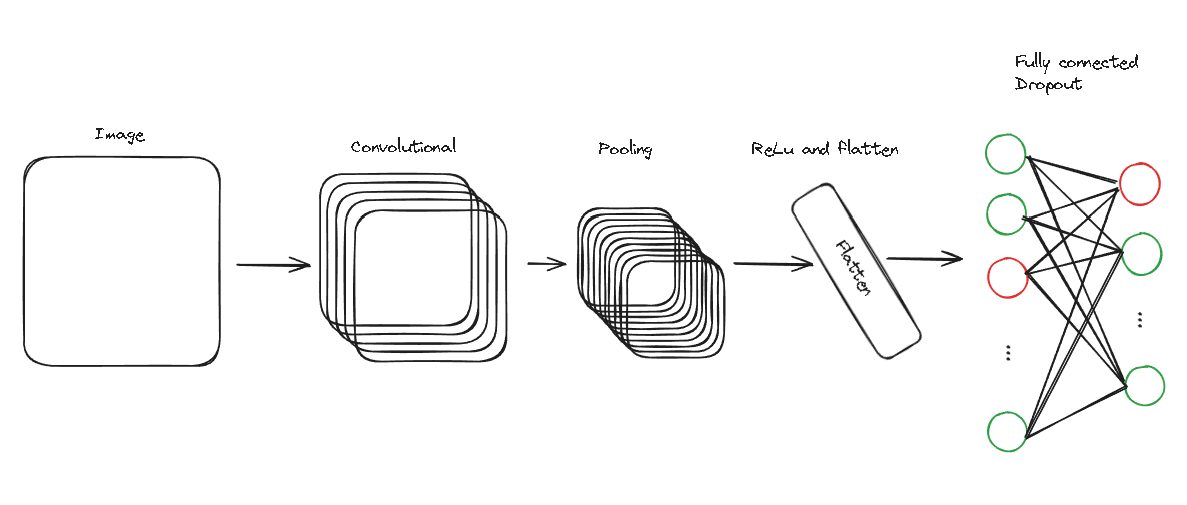
\includegraphics[width=\linewidth]{network}

    \subsubsection{Convolutional layers}
    This is the most important layer in a standard CNN model.
    The purpose of a convolutional layer in a Convolutional Neural Network (CNN) is to extract features from the input data. 
    This layer performs a mathematical operation called convolution, 
    which involves sliding a filter (also known as a kernel) over the input data to produce a feature map.\cite{o4}\\
    The most common type of convolution that is used is the 2D convolution layer and is usually abbreviated as conv2D. 
    A filter or a kernel in a conv2D layer “slides” over the 2D input data, performing an elementwise multiplication. 
    As a result, it will be summing up the results into a single output pixel. 
    The kernel will perform the same operation for every location it slides over, transforming a 2D matrix of features into a different 2D matrix of features.\cite{o5}
    \subsubsection{Non Linearity (Activation) layers}
    Next, we have the activation layer.
    An activation layer is a crucial component that introduces non-linearity into the network. 
    This is important because convolution operations are linear, and without non-linearity, the network would not be able to model complex data distributions effectively.
    \subsubsection{Pooling layers}
    Pooling layers are used to reduce the spatial dimensions of the input volume.
    They divide the input data into small regions, called pooling windows or receptive fields, 
    and perform an aggregation operation, such as taking the maximum or average value, within each window. 
    This aggregation reduces the size of the feature maps, resulting in a compressed representation of the input data.\cite{o7}
    \subsubsection{Fully connected layers}
    A fully connected layer refers to a neural network in which each neuron applies a linear transformation to the input vector through a weights matrix. 
    As a result, all possible connections layer-to-layer are present, meaning every input of the input vector influences every output of the output vector.\cite{o8}
    \subsubsection{Dropout layers}
    Dropout is a regularization technique that helps prevent overfitting by randomly setting a fraction of the input units to zero during training.
    This method makes the model more robust and less likely to memorize the training data.
    \subsubsection{Flatten layers}
    The flatten layer typically appears after the convolutional and pooling layers in convolutional neural network (CNN) architectures. 
    It acts as a bridge between the convolutional/pooling layers, which extract spatial features, 
    and the fully connected layers, which perform classification or regression tasks.\cite{o10}
    \subsubsection{Softmax layers}
    The Softmax function essentially converts the raw output scores (logits) of the neural network into probabilities. 
    This allows the network to output a probability distribution over the classes, 
    making it easier to interpret the model's predictions and make decisions based on the class probabilities.
    In a CNN, the Softmax function is typically applied to the output of the last fully connected layer of the network, 
    which is then used to make predictions about the input data belonging to different classes.\cite{o11}
    \subsubsection{Batch normalization layers}
    Batch Normalization is a normalization technique that can be applied at the layer level. 
    Put simply, it normalizes “the inputs to each layer to a learnt representation likely close to ( $\mu$ = 0.0, $\sigma$ = 1.0). 
    As a consequence, all the layer inputs are normalized, and significant outliers are less likely to impact the training process in a negative way. 
    And if they do, their impact will be much lower than without using Batch Normalization.\cite{o17}
    This is done when the data is not normalized, and the model is not converging well.
    For instance if the batches are different from each other, causing the weights of the model to shift from eachother, making the training process longer. 
    \subsection{Pixel}
    The first method we used to train our model is by using the pixels of the image.
    \subsubsection{Network}
    The model we created is a Convolutional Neural Network (CNN) model.
    We have several layers to form our network. 
    We have 3 convolutional layers, 3 max pooling layers, 4 activation layers, 2 fully connected layers, 2 dropout layers, 1 flatten layer and one softmax.

    The network is structured as follows:\\
    The input shape of our model is (28, 28, 1) and the output shape is the number of classes we have, which is 24 (for the 24 letters of the alphabet excluding j and z).
    We insert the image first through a convolutional layer, this outputs a feature map, with 32 output channels.
    We then apply an activation layer to introduce some non-linearity.
    After that we apply some dropout to prevent overfitting (or at least try).
    We then apply a max pooling layer to reduce the spatial dimensions of the input volume. This reduces the size of the feature maps to 14$\times$14.
    We then repeat the process two more times with the next convolutional layer, activation layer, dropout layer and max pooling layer.
    In the end, we have a 128$\times$3$\times$3 feature map. We then flatten this feature map to a 1152$\times$1 vector.
    We then apply a fully connected layer to this vector, then another fully connected layer, with some additional layers in between.
    Finally, we apply a softmax layer to get the probabilities of each class.
    TODO NEEDS TO CHANGE
    
    \subsection{Landmarks}
    The second method we used to train our model is by using the landmarks of the hand.
    \subsubsection{Network}
    Again, we make use of a CNN model.
    The network is structured as follows:\\
    TODO

    \subsection{Training and Validation}
    Next, we will discuss how we trained our model.
    Training is similar to the training of any other model.
    We define some hyperparameters, such as the learning rate, the number of epochs, the batch size, etc.
    More on that later.
    We then feed the training data to the model and let it train.
    This training process is done in batches, where the model is fed a batch of data, computes the loss, and updates the weights.
    During every epoch, we have two passes through the data, one forward pass and one backward pass. 
    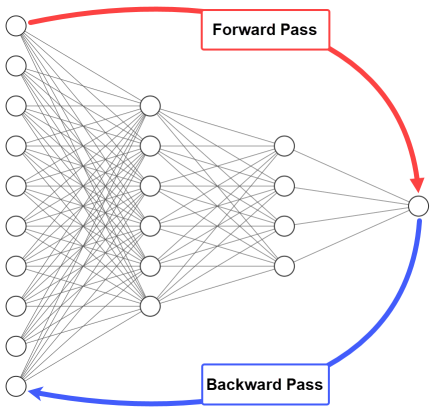
\includegraphics[width=\linewidth]{Backpropagation-passes-architecture}
    The purpose of the forward pass is to propagate input data through the network and produce predictions or outputs based on the model's learned parameters (weights and biases).\cite{o13}
    In the backward pass, the flow is reversed so that we start by propagating the error to the output layer until reaching the input layer passing through the hidden layers.\cite{o14}
    After these two passes, we have completed one epoch for training.

    We also have a validation set, which is used to evaluate the model's performance on unseen data.
    Note that in our case, the validation set is a subset of the original training set that we split up in training and validation.

    After these two steps are done, we evaluate the model based on the performances of training and validation.
    The training can be interupted if the model is not improving anymore.
    We do this by using a technique called early stopping.
    Early stopping works as follows:
    We monitor the validation loss and trainig loss during training. 
    At each epoch, we check if the validation loss has decreased compared to the training loss.
    In case the validation loss has not decreased for a certain number of epochs, we stop the training process.
    The amount of epochs we wait before stopping is a hyperparameter we call patience.
    Why do we use early stopping?
    Early stopping is a regularization technique that helps prevent overfitting by stopping the training process before the model starts to memorize the training data.\cite{o15}
    \subsubsection{Tuning}
    We also have some hyperparameters that we can tune.
    Earlier we already mentioned some hyperparameters, but what are hyperparameters?
    They are like settings you choose before teaching a neural network to do a task. 
    They control things like how many layers the network has, how quickly it learns, and how it adjusts its internal values.\cite{o16}
    Some hyperparameters we can tune are:
    \begin{itemize}
        \item Learning rate
        \item Number of epochs
        \item Batch size
        \item etc.
    \end{itemize}
    These hyperparameters can be tuned based on how the model is performing after training.
    In case the learning takes to long and the model is not improving, we can increase the learning rate for instance.

    Hyperparameters are important because they can have a significant impact on the performance of the model.
    In practice, hyperparameters are usually set based on trial and error, 
    where different values are tested to see which ones produce the best results on a validation set.

\end{document}
